\chapter{Psalm 6}

\begin{figure}
  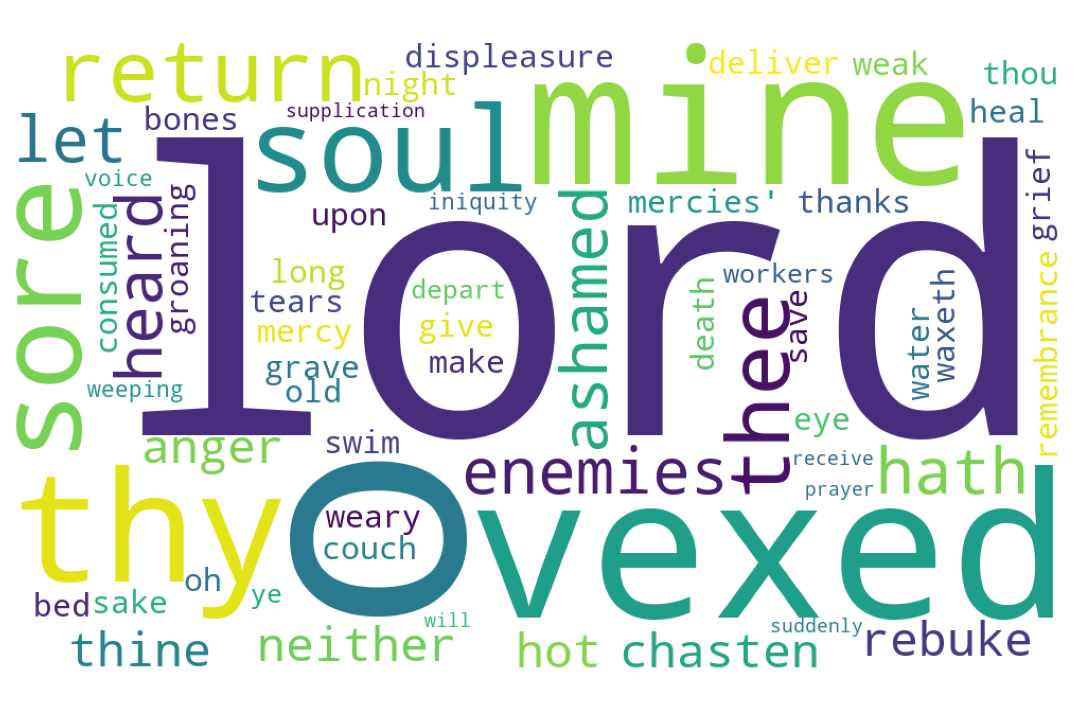
\includegraphics[width=\linewidth]{19OT-Psalms/Psalm6-WordCloud.jpg}
  \caption{Psalm 6 Word Cloud}
  \label{fig:Psalm 6 word Cloud}
\end{figure}

\marginpar{\scriptsize \centering \fcolorbox{bone}{lime}{\textbf{WHEN GOD IS NEAR}}\\ (Psalm 6:1-10) 
\begin{compactenum}[I.][8]
    \item \textbf{Recognize Sin and its Damage}  \index[scripture]{Psalms!Psa 006:02} (Psa 6:2)
    \item \textbf{Reach a State of Despair} \index[scripture]{Psalms!Psa 006:03} (Psa 6:3)
    \item \textbf{Remember the Source of his Deliverance} \index[scripture]{Psalms!Psa 006:04} (Psa 6:4)
    \item \textbf{Repeat his Sorrow and Distress} \index[scripture]{Psalms!Psa 006:06} (Psa 6:6)
    \item \textbf{Recount the Sum of Adversaries} \index[scripture]{Psalms!Psa 006:07} (Psa 6:7)
    \item \textbf{Request for Sinners to Depart} \index[scripture]{Psalms!Psa 006:08} (Psa 6:8)
    \item \textbf{Rejoice in the Savior and Deliverer} \index[scripture]{Psalms!Psa 006:09} (Psa 6:9)
\end{compactenum} } 

\marginpar{\scriptsize \centering \fcolorbox{bone}{yellow}{\textbf{THE PSALMIST'S SITUATION}}\\ (Psalm 6:1-10) 
\begin{compactenum}[I.][8]
     \item Acknowledges the \textbf{Sinner Deserves God's Anger}  \index[scripture]{Psalms!Psa 006:01} (Psa 6:1)
    \item Acknowledges the \textbf{Sinner has Earned God's Displeasure}  \index[scripture]{Psalms!Psa 006:01} (Psa 6:1)
    \item He \textbf{Is Desiring Mercy}  \index[scripture]{Psalms!Psa 006:02} (Psa 6:2)
    \item Knows God \textbf{Can Deliver Souls}  \index[scripture]{Psalms!Psa 006:04} (Psa 6:4)
    \item Knows The \textbf{Dead have no Hope}  \index[scripture]{Psalms!Psa 006:05} (Psa 6:5)
    \item Chooses to \textbf{Depart} from Sinners \index[scripture]{Psalms!Psa 006:08} (Psa 6:8)
    \item \textbf{Depends} on God's Reponses \index[scripture]{Psalms!Psa 006:09} (Psa 6:9)
\end{compactenum} } 

\footnote{\textcolor[cmyk]{0.99998,1,0,0}{\hyperlink{TOC}{Return to end of Table of Contents.}}}\footnote{\href{https://audiobible.com/bible/bible.html}{\textcolor[cmyk]{0.99998,1,0,0}{Psalms Audio}}}\textcolor[cmyk]{0.99998,1,0,0}{To the chief musician on Neginoth upon Sheminith. A Psalm of David.}\\
\\
\textcolor[cmyk]{0.99998,1,0,0}{O LORD, rebuke me not in thine anger, neither chasten me in thy hot displeasure.}
[2] \textcolor[cmyk]{0.99998,1,0,0}{Have mercy upon me, O LORD; for I \emph{am} weak: O LORD, heal me; for my bones are vexed.}
[3] \textcolor[cmyk]{0.99998,1,0,0}{My soul is also sore vexed: but thou, O LORD, how long?}
[4] \textcolor[cmyk]{0.99998,1,0,0}{Return, O LORD, deliver my soul: oh save me for thy mercies' sake.}
[5] \textcolor[cmyk]{0.99998,1,0,0}{For in death \emph{there} \emph{is} no remembrance of thee: in the grave who shall give thee thanks?}
[6] \textcolor[cmyk]{0.99998,1,0,0}{I am weary with my groaning; all the night make I my bed to swim; I water my couch with my tears.}
[7] \textcolor[cmyk]{0.99998,1,0,0}{Mine eye is consumed because of grief; it waxeth old because of all mine enemies.}
[8] \textcolor[cmyk]{0.99998,1,0,0}{Depart from me, all ye workers of iniquity; for the LORD hath heard the voice of my weeping.}
[9] \textcolor[cmyk]{0.99998,1,0,0}{The LORD hath heard my supplication; the LORD will receive my prayer.}
[10] \textcolor[cmyk]{0.99998,1,0,0}{Let all mine enemies be ashamed and sore vexed: let them return \emph{and} be ashamed suddenly.}



